\newpage\handout
{Drill Problems: Week 03-7}
{\textsc{Scholastic Aptitude Test (SAT)}}
{\href{https://creativecommons.org/licenses/by-nc-sa/4.0/}{CC BY-NC-SA 4.0 license}}
{Author: Jaehoon Song}{Release: \generatedOn}
{SAT: Drill Problems}
% Copyright & Disclaimer
\newcommand{\BookAuthor}{Jaehoon Song (Lecturer)}

\begin{center}
  \begin{minipage}{0.85\textwidth}
    {\small\textbf{Purpose and Usage:}}\\[0.2cm]
    {\footnotesize
    This material has been developed for internal training and educational 
    purposes at Hans edu LLC. It is intended for use within our organization 
    and should not be distributed, sold, or used for commercial purposes 
    outside of our educational programs.}\\[0.5cm]
    
    {\small\textbf{For Our Community:}}\\[0.2cm]
    {\footnotesize
    Students and staff are welcome to use this material in their studies and 
    teaching at Hans edu LLC. While we encourage active engagement with the 
    content, please respect that this is proprietary material. Any 
    reproduction or distribution outside of our organization's educational 
    activities is not permitted.}\\[0.5cm]
    
    {\small\textbf{Content and Attribution:}}\\[0.2cm]
    {\footnotesize
    This material represents our adaptation of various established mathematics 
    textbooks, reorganized and enhanced for our teaching context. While we've 
    added our own pedagogical improvements, we maintain proper attribution to 
    original sources. This work is shared under the Creative Commons 
    Attribution-NonCommercial-ShareAlike (CC BY-NC-SA) license, allowing 
    internal use and adaptation while respecting the original creators' rights.\\[0.2cm]
    \small Key Permissions under CC BY-NC-SA 4.0:
    \begin{itemize}
      \item credit the creator.
      \item no commercial use.
      \item new creations must carry the same license.
      \item copy and redistribute the material in any medium or format
      \item remix, transform, and build upon the material
    \end{itemize}}
    % Some content may be derived from sources under the CC0 1.0 Universal 
    % license, which allows for free use, modification, and distribution.}\\[0.5cm]
    {\small\textbf{Quality Assurance:}}\\[0.2cm]
    {\footnotesize
    We have carefully reviewed this material for accuracy and clarity. However, 
    as with any educational resource, we encourage critical engagement and 
    verification of concepts. If you notice any issues or have suggestions for 
    improvement, please bring them to our attention.}
  \end{minipage}
  \vspace{2cm} \\
  {\small © \the\year\ Hans edu LLC. All rights reserved.}\\[0.5cm]
  {\small Written by \BookAuthor}\\[1cm]
\end{center}

\newpage


\begin{enumerate}
  \item \textbf{X-Intercept} (10 points)\\
  The $x$-intercept of the graph shown is $(x, 0)$. What is the value of $x$?
  \insertimage{0.40}{images/2025_06_15_5ccb8dd1752fe76599e7g-021}{reference attached}
  \begin{subanswer}
    % your answer here
  \end{subanswer}
  

  \newpage


  \item \textbf{Graph Equation} (10 points)\\
  Which of the following could be the equation of the graph shown in the $xy$-plane?
  \insertimage{0.40}{images/2025_06_15_5ccb8dd1752fe76599e7g-022}{reference attached}
  \begin{enumerate}[label=(\Alph*)]
    \item $y=-\frac{1}{10} x(x-4)(x+5)$
    \item $y=-\frac{1}{10} x(x-4)(x+5)^{2}$
    \item $y=-\frac{1}{10} x(x-5)(x+4)$
    \item $y=-\frac{1}{10} x (x-5)^{2}(x+4)$
  \end{enumerate}
  \begin{subanswer}
    % your answer here
  \end{subanswer}


  \item \textbf{Function Translation} (10 points)\\
  $$f(x)=4 x^{2}+64 x+262$$\\
  The function $g$ is defined by $g(x)=f(x+5)$. For what value of $x$ does $g(x)$ reach its minimum?
  \begin{enumerate}[label=(\Alph*)]
    \item -13
    \item -8
    \item -5
    \item -3
  \end{enumerate}
  \begin{subanswer}
    % your answer here
  \end{subanswer}


  \newpage

  \item \textbf{Polynomial Roots} (10 points)\\
  The graph of $y=f(x)$ is shown, where the function $f$ is defined by $f(x)=a x^{3}+b x^{2}+c x+d$ and $a, b, c$, and $d$ are constants. For how many values of $x$ does $f(x)=0$?
  \insertimage{0.40}{images/2025_06_15_5ccb8dd1752fe76599e7g-024}{reference attached}
  \begin{enumerate}[label=(\Alph*)]
    \item One
    \item Two
    \item Three
    \item Four
  \end{enumerate}
  \begin{subanswer}
    % your answer here
  \end{subanswer}

  \newpage

  \item \textbf{Data Representation} (10 points)\\
  The table shown includes some values of $x$ and their corresponding values of $y$.
  \begin{center}
    \begin{tabular}{|c|c|}
      \hline
      $x$ & $y$ \\
      \hline
      0 & 0 \\
      \hline
      1 & 1 \\
      \hline
      2 & 8 \\
      \hline
      3 & 27 \\
      \hline
    \end{tabular}
  \end{center}
  Which of the following graphs in the $xy$-plane could represent the relationship between $x$ and $y$?
  \begin{center}
    \begin{tabular}{cccc}
      A. & B. & C. & D. \\
      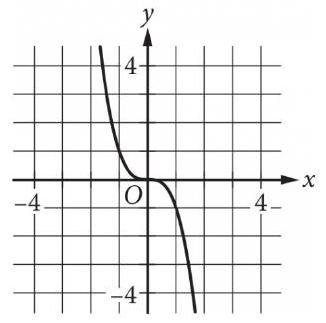
\includegraphics[width=0.23\textwidth]{images/2025_06_15_5ccb8dd1752fe76599e7g-025(2)} &
      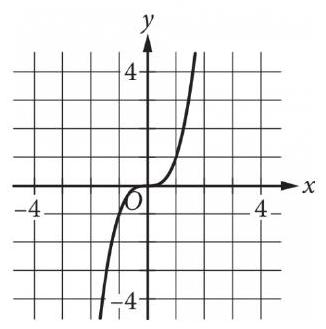
\includegraphics[width=0.23\textwidth]{images/2025_06_15_5ccb8dd1752fe76599e7g-025} &
      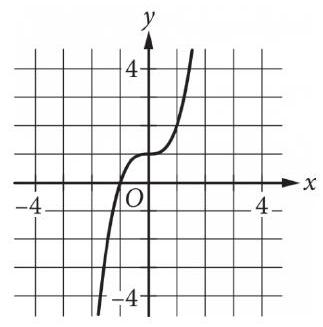
\includegraphics[width=0.23\textwidth]{images/2025_06_15_5ccb8dd1752fe76599e7g-025(3)} &
      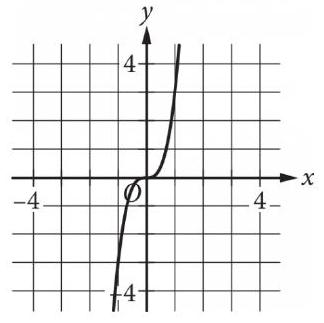
\includegraphics[width=0.23\textwidth]{images/2025_06_15_5ccb8dd1752fe76599e7g-025(1)} \\
    \end{tabular}
  \end{center}
  \begin{subanswer}
    % your answer here
  \end{subanswer}

  \item \textbf{Function Translation} (10 points)\\
  The function $f$ is defined by $f(x)=(x-6)(x-2)(x+6)$. In the $xy$-plane, the graph of $y=g(x)$ is the result of translating the graph of $y=f(x)$ up 4 units. What is the value of $g(0)$?
  \begin{subanswer}
    % your answer here
  \end{subanswer}

  \item \textbf{Rectangle Area} (10 points)\\
  A rectangle has a length of $x$ units and a width of $(x-15)$ units. If the rectangle has an area of 76 square units, what is the value of $x$?
  \begin{enumerate}[label=(\Alph*)]
    \item 4
    \item 19
    \item 23
    \item 76
  \end{enumerate}
  \begin{subanswer}
    % your answer here
  \end{subanswer}

  \item \textbf{Exponential Growth} (10 points)\\
  A scientist initially measures 12,000 bacteria in a growth medium. 4 hours later, the scientist measures 24,000 bacteria. Assuming exponential growth, the formula $P=C(2)^{rt}$ gives the number of bacteria in the growth medium, where $r$ and $C$ are constants and $P$ is the number of bacteria $t$ hours after the initial measurement. What is the value of $r$?
  \begin{enumerate}[label=(\Alph*)]
    \item $\frac{1}{12,000}$
    \item $\frac{1}{4}$
    \item 4
    \item 12,000
  \end{enumerate}
  \begin{subanswer}
    % your answer here
  \end{subanswer}

  \item \textbf{Projectile Motion} (10 points)\\
  A quadratic function models a projectile's height, in meters, above the ground in terms of the time, in seconds, after it was launched. The model estimates that the projectile was launched from an initial height of 7 meters above the ground and reached a maximum height of 51.1 meters above the ground 3 seconds after the launch. How many seconds after the launch does the model estimate that the projectile will return to a height of 7 meters?
  \begin{enumerate}[label=(\Alph*)]
    \item 3
    \item 6
    \item 7
    \item 9
  \end{enumerate}
  \begin{subanswer}
    % your answer here
  \end{subanswer}

  \item \textbf{Quadratic Minimum} (10 points)\\
  The given equation relates the variables $x$ and $y$:
  \[
    y=x^{2}-14x+22
  \]
  For what value of $x$ does the value of $y$ reach its minimum?
  \begin{subanswer}
    % your answer here
  \end{subanswer}

  \newpage

  \item \textbf{Polynomial Simplification} (10 points)\\
  Which expression is equivalent to $11x^{3}-5x^{3}$?
  \begin{enumerate}[label=(\Alph*)]
    \item $16x^{3}$
    \item $6x^{3}$
    \item $6x^{6}$
    \item $16x^{6}$
  \end{enumerate}
  \begin{subanswer}
    % your answer here
  \end{subanswer}

  \item \textbf{Polynomial Addition} (10 points)\\
  Which expression is equivalent to $50x^{2}+5x^{2}$?
  \begin{enumerate}[label=(\Alph*)]
    \item $250x^{2}$
    \item $10x^{2}$
    \item $45x^{2}$
    \item $55x^{2}$
  \end{enumerate}
  \begin{subanswer}
    % your answer here
  \end{subanswer}

  \item \textbf{Polynomial Multiplication} (10 points)\\
  The expression $(3x-23)(19x+6)$ is equivalent to the expression $ax^{2}+bx+c$, where $a$, $b$, and $c$ are constants. What is the value of $b$?
  \begin{subanswer}
    % your answer here
  \end{subanswer}

  \item \textbf{Expression Simplification} (10 points)\\
  Which expression is equivalent to $20w-(4w+3w)$?
  \begin{enumerate}[label=(\Alph*)]
    \item $10w$
    \item $13w$
    \item $19w$
    \item $21w$
  \end{enumerate}
  \begin{subanswer}
    % your answer here
  \end{subanswer}


  \newpage

  \item \textbf{Rational Expression} (10 points)\\
  Which expression is equivalent to $\frac{4}{4x-5}-\frac{1}{x+1}$?
  \begin{enumerate}[label=(\Alph*)]
    \item $\frac{1}{(x+1)(4x-5)}$
    \item $\frac{3}{3x-6}$
    \item $-\frac{1}{(x+1)(4x-5)}$
    \item $\frac{9}{(x+1)(4x-5)}$
  \end{enumerate}
  \begin{subanswer}
    % your answer here
  \end{subanswer}

  \item \textbf{Linear Expression} (10 points)\\
  Which of the following is equivalent to $3(x+5)-6$?
  \begin{enumerate}[label=(\Alph*)]
    \item $3x-3$
    \item $3x-1$
    \item $3x+9$
    \item $15x-6$
  \end{enumerate}
  \begin{subanswer}
    % your answer here
  \end{subanswer}

  \item \textbf{Rational Expression} (10 points)\\
  In the expression $$\frac{x^{2}-c}{x-b}$$, $b$ and $c$ are positive integers. If the expression is equivalent to $x+b$ and $x \neq b$, which of the following could be the value of $c$?
  \begin{enumerate}[label=(\Alph*)]
    \item 4
    \item 6
    \item 8
    \item 10
  \end{enumerate}
  \begin{subanswer}
    % your answer here
  \end{subanswer}

  \newpage

  \item \textbf{Radical Expression} (10 points)\\
  Which of the following expressions is equivalent to $\sqrt[3]{x^3y^6}$?
  \begin{enumerate}[label=(\Alph*)]
    \item $y^{2}$
    \item $xy^{2}$
    \item $y^{3}$
    \item $xy^{3}$
  \end{enumerate}
  \begin{subanswer}
    % your answer here
  \end{subanswer}

  \item \textbf{Polynomial Multiplication} (10 points)\\
  Which expression is equivalent to $(d-6)(8d^{2}-3)$?
  \begin{enumerate}[label=(\Alph*)]
    \item $8d^{3}-14d^{2}-3d+18$
    \item $8d^{3}-17d^{2}+48$
    \item $8d^{3}-48d^{2}-3d+18$
    \item $8d^{3}-51d^{2}+48$
  \end{enumerate}
  \begin{subanswer}
    % your answer here
  \end{subanswer}

  \item \textbf{Square Difference} (10 points)\\
  If $x^{2}=a+b$ and $y^{2}=a+c$, which of the following is equal to $(x^{2}-y^{2})^{2}$?
  \begin{enumerate}[label=(\Alph*)]
    \item $a^{2}-2ac+c^{2}$
    \item $b^{2}-2bc+c^{2}$
    \item $4a^{2}-4abc+c^{2}$
    \item $4a^{2}-2abc+b^{2}c^{2}$
  \end{enumerate}
  \begin{subanswer}
    % your answer here
  \end{subanswer}

  \item \textbf{System of Equations} (10 points)\\
  If the ordered pair $(x,y)$ satisfies the system of equations
  \[
    \begin{aligned}
      & y=x^{2}-4x+4 \\
      & y=4-x
    \end{aligned}
  \]
  what is one possible value of $x$?
  \begin{subanswer}
    % your answer here
  \end{subanswer}

  \newpage

  \item \textbf{Wave Equation} (10 points)\\
  An oceanographer uses the equation $$s=\frac{3}{2}p$$ to model the speed $s$, in knots, of an ocean wave, where $p$ represents the period of the wave, in seconds. Which of the following represents the period of the wave in terms of the speed of the wave?
  \begin{enumerate}[label=(\Alph*)]
    \item $p=\frac{2}{3}s$
    \item $p=\frac{3}{2}s$
    \item $p=\frac{2}{3}+s$
    \item $p=\frac{3}{2}+s$
  \end{enumerate}
  \begin{subanswer}
    % your answer here
  \end{subanswer}

  \item \textbf{Quadratic Equation} (10 points)\\
  Which of the following is a solution to the equation $2x^{2}-4=x^{2}$?
  \begin{enumerate}[label=(\Alph*)]
    \item 1
    \item 2
    \item 3
    \item 4
  \end{enumerate}
  \begin{subanswer}
    % your answer here
  \end{subanswer}

  \item \textbf{Linear Equation} (10 points)\\
  The given equation relates the positive numbers $q$, $r$, and $s$:
  \[
    q-29r=s
  \]
  Which equation correctly expresses $q$ in terms of $r$ and $s$?
  \begin{enumerate}[label=(\Alph*)]
    \item $q=s-29r$
    \item $q=s+29r$
    \item $q=29rs$
    \item $q=-\frac{s}{29r}$
  \end{enumerate}
  \begin{subanswer}
    % your answer here
  \end{subanswer}

  \newpage

  \item \textbf{Quadratic Solutions} (10 points)\\
  In the given equation, $a$ and $b$ are positive constants:
  \[
    57x^{2}+(57b+a)x+ab=0
  \]
  The product of the solutions to the given equation is $kab$, where $k$ is a constant. What is the value of $k$?
  \begin{enumerate}[label=(\Alph*)]
    \item $\frac{1}{57}$
    \item $\frac{1}{19}$
    \item 1
    \item 57
  \end{enumerate}
  \begin{subanswer}
    % your answer here
  \end{subanswer}

  \item \textbf{Quadratic No Solutions} (10 points)\\
  In the given equation, $b$ is a positive integer:
  \[
    -x^{2}+bx-676=0
  \]
  The equation has no real solution. What is the greatest possible value of $b$?
  \begin{subanswer}
    % your answer here
  \end{subanswer}

  \item \textbf{Rational Equation} (10 points)\\
  The given equation relates the distinct positive numbers $p$, $k$, and $j$:
  \[
    p=\frac{k}{4j+9}
  \]
  Which equation correctly expresses $4j+9$ in terms of $p$ and $k$?
  \begin{enumerate}[label=(\Alph*)]
    \item $4j+9=\frac{k}{p}$
    \item $4j+9=kp$
    \item $4j+9=k-p$
    \item $4j+9=\frac{p}{k}$
  \end{enumerate}
  \begin{subanswer}
    % your answer here
  \end{subanswer}

  \item \textbf{Quadratic Expression} (10 points)\\
  If $3x^{2}-18x-15=0$, what is the value of $x^{2}-6x$?
  \begin{subanswer}
    % your answer here
  \end{subanswer}

  \item \textbf{Intersection Point} (10 points)\\
  In the $xy$-plane, what is the $y$-coordinate of the point of intersection of the graphs of $y=(x-1)^{2}$ and $y=2x-3$?
  \begin{subanswer}
    % your answer here
  \end{subanswer}

  \item \textbf{Quadratic No Solutions} (10 points)\\
  In the equation $2x^{2}-4x=t$, $t$ is a constant. If the equation has no real solutions, which of the following could be the value of $t$?
  \begin{enumerate}[label=(\Alph*)]
    \item -3
    \item -1
    \item 1
    \item 3
  \end{enumerate}
  \begin{subanswer}
    % your answer here
  \end{subanswer}
\end{enumerate}

